%  Μεταγλώττιση με XeLaTeX

\documentclass{llncs}
\pagestyle{headings} 
%
\usepackage{makeidx}  % allows for indexgeneration
%
\usepackage{xltxtra}
\usepackage{xgreek}

\usepackage{caption}
\usepackage{subcaption}

\setsansfont{Arial}
\setmonofont{Courier New}
\setmainfont[Mapping=tex-text]{Times New Roman}
% \setmainfont[Mapping=tex-text]{GFS Didot} 
% \setsansfont{GFS Didot}
% \setmonofont{GFS Didot}

\renewcommand{\abstractname}{Περίληψη}
\newtheorem{observation}{Παρατήρηση}
\renewcommand{\keywordname}{\bf Λέξεις Κλειδιά:}
\renewcommand\refname{Αναφορές}
\renewcommand\ackname{Ευχαριστίες}
\renewcommand\andname{και}
\renewcommand\corollaryname{Πόρισμα}
\renewcommand\definitionname{Ορισμός}
\renewcommand\examplename{Παράδειγμα}
\renewcommand\exercisename{Άσκηση}
\renewcommand\figurename{Εικ.}
\renewcommand\lemmaname{Λήμμα}
\renewcommand\proofname{Απόδειξη}
\renewcommand\propositionname{Πρόταση}
\renewcommand\solutionname{Λύση}
\renewcommand\tablename{Πίνακας}
\renewcommand\theoremname{Θεώρημα}

\begin{document}
%
\title{\Huge Προγραμματιστική Εργασία Πρόβλεψη κόστους ασφάλισης οχημάτων}
%
%
\author{\Large Χαρά Τσίρκα \and Πρόδρομος Αβραμίδης \and Γεώργιος Γεροντίδης}
%
%
%
\institute{\email{\{ctsirka, pavramidis, ggerontidis\}@e-ce.uth.gr}\\
8$^{ο}$ εξάμηνο\\
\begin{center}
    \vspace{1cm}
    
\includegraphics[width=0.4\textwidth]{uthlogo.png}
    \vspace{1cm}
\end{center}
\Large Τμήμα Ηλεκτρολόγων Μηχανικών \& Μηχανικών Υπολογιστών\\
Πανεπιστήμιο Θεσσαλίας, Βόλος\\
\vspace{1cm}
{\bf \Large Εξόρυξη Δεδομένων 2023-24}\\
\Large Διδάσκον: Μ.Βασιλακόπουλος\\
\vspace{1cm}
Μάιος 2024}

\maketitle



\begin{abstract}
    Η εργασία μας επικεντρώνεται στην πρόβλεψη του κόστους ασφάλισης μηχανοκίνητων οχημάτων. Η ανάλυση αυτή αποτελεί ένα κρίσιμο ζήτημα στον τομέα της ασφάλισης, καθώς επιτρέπει στους ασφαλιστές να προσδιορίζουν με μεγαλύτερη ακρίβεια τα ασφαλιστικά ασφάλιστρα, λαμβάνοντας υπόψη διάφορους παράγοντες που επηρεάζουν το κόστος.
    Η διαδικασία της εργασίας ξεκινά με την προ-επεξεργασία των δεδομένων, κατά την οποία πραγματοποιήθηκε εξερευνητική ανάλυση (exploratory analysis) για τον προσδιορισμό των κριτηρίων διαχωρισμού των δεδομένων. Κατά τη διάρκεια αυτής της ανάλυσης, μετρήθηκε ο βαθμός επίδρασης κάθε χαρακτηριστικού (feature) του συνόλου δεδομένων στα αποτελέσματα. Με τη βοήθεια διαγραμμάτων, καταφέραμε να επιλέξουμε τον κατάλληλο διαχωρισμό των δεδομένων για περαιτέρω ανάλυση.
    Στη συνέχεια, η εργασία θα προχωρήσει στη δημιουργία και αξιολόγηση των μοντέλων πρόβλεψης, λαμβάνοντας υπόψη την είσοδο των χρηστών, ενώ θα ακολουθήσει η οπτικοποίηση και η αξιολόγηση των αποτελεσμάτων.
\end{abstract}


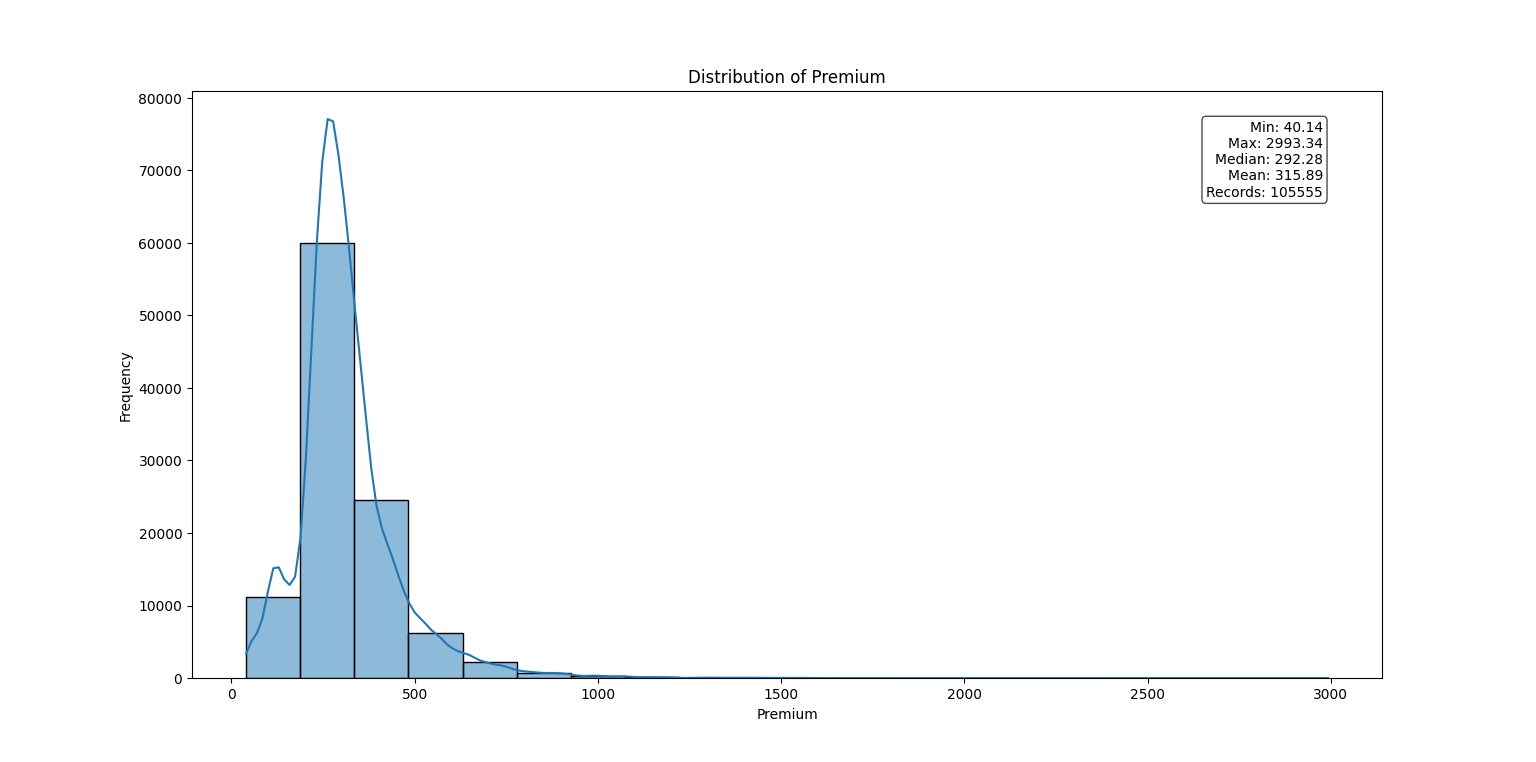
\includegraphics[width=0.7\textwidth, keepaspectratio]{images/premium.png}


\begin{figure}
    \centering
     \begin{subfigure}{0.45\linewidth}
      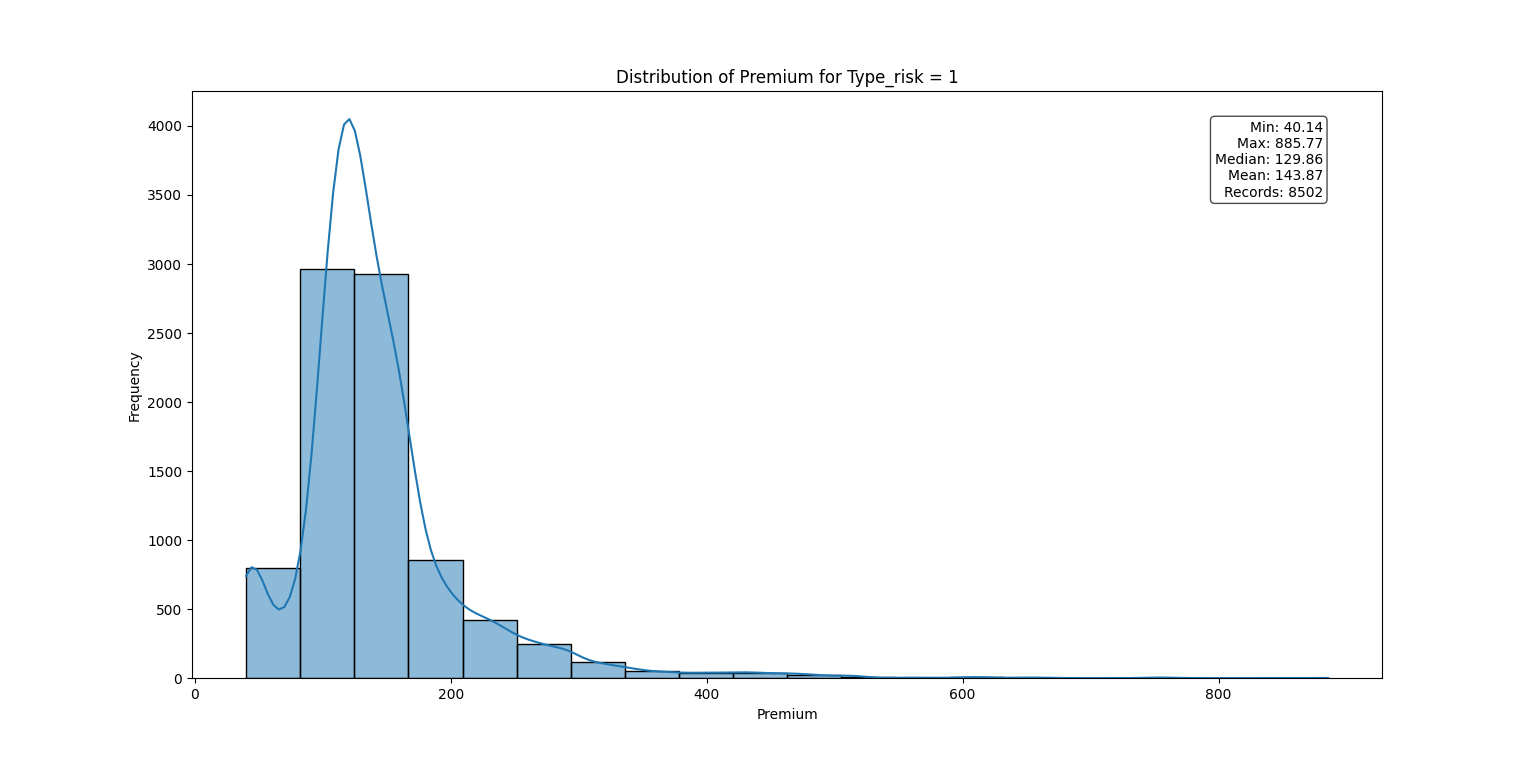
\includegraphics[width=\linewidth]{images/premium_risk1.png}
      \caption{Motorbikes}
      \label{fig:subfig1}
     \end{subfigure}
     \begin{subfigure}{0.45\linewidth}
      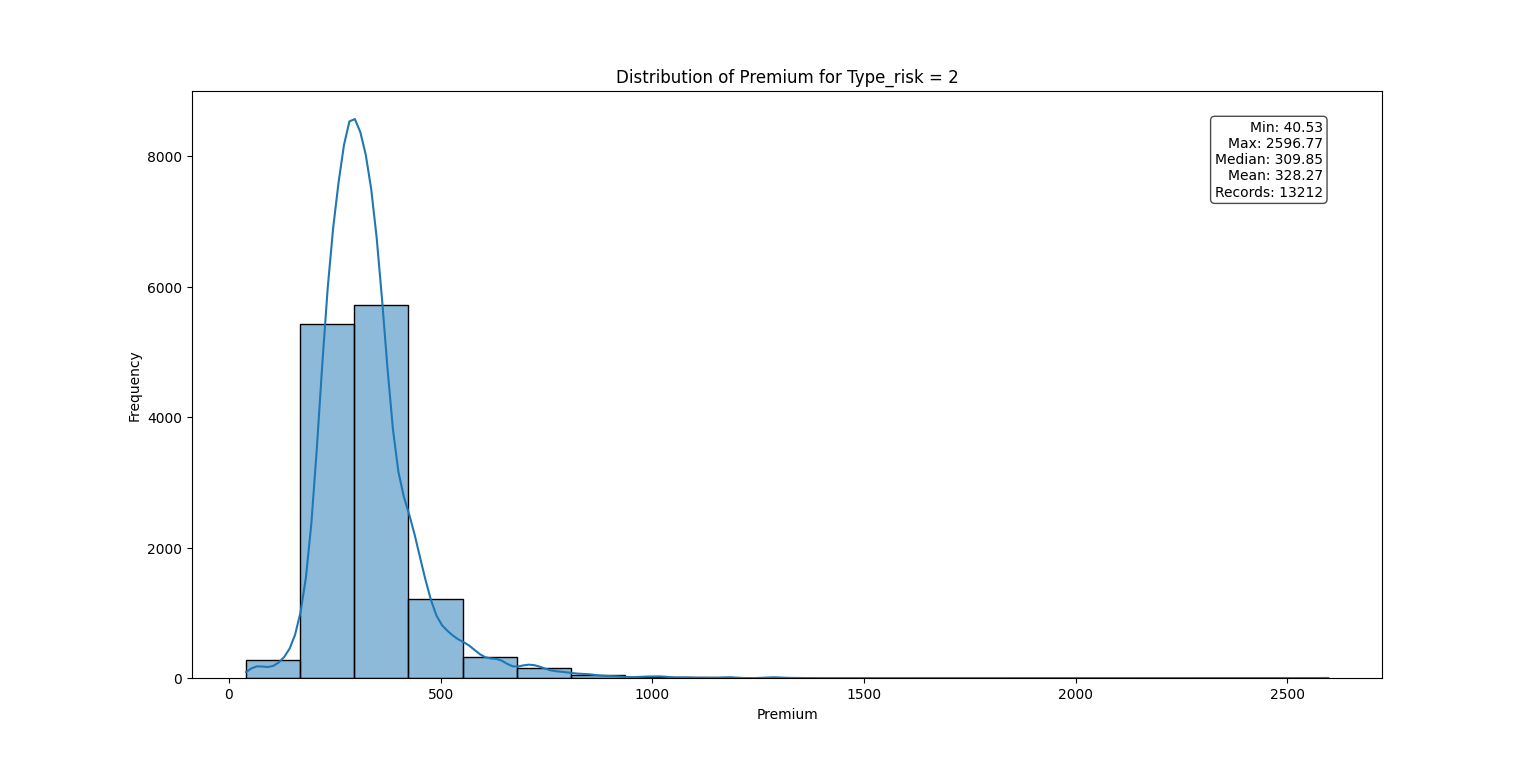
\includegraphics[width=\linewidth]{images/premium_risk2.png}
      \caption{Vans}
      \label{fig:subfig2}
      \end{subfigure}
  \vfill
       \begin{subfigure}{0.45\linewidth}
       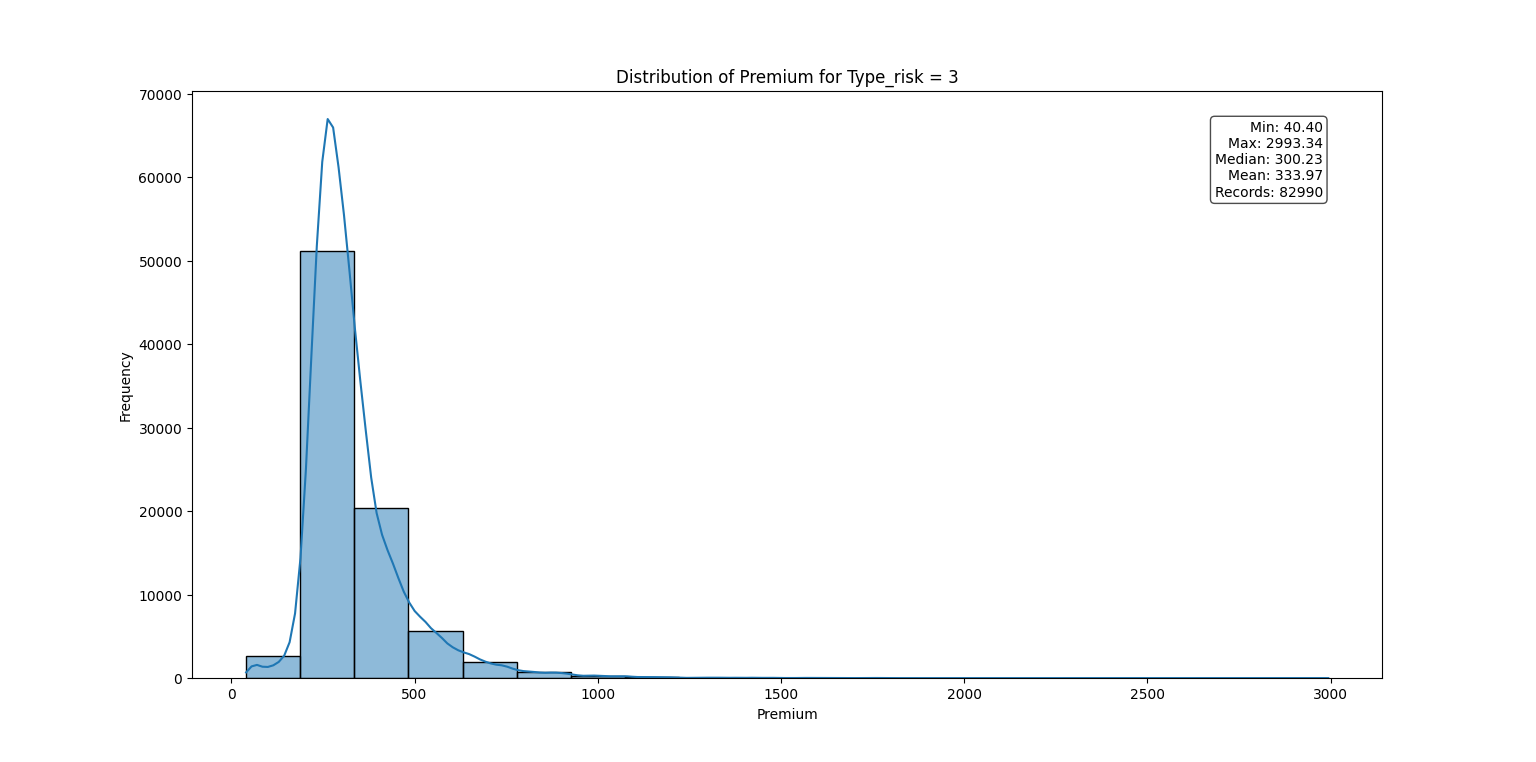
\includegraphics[width=\linewidth]{images/premium_risk3.png}
       \caption{Passenger cars}
       \label{fig:subfig3}
        \end{subfigure}
         \begin{subfigure}{0.45\linewidth}
        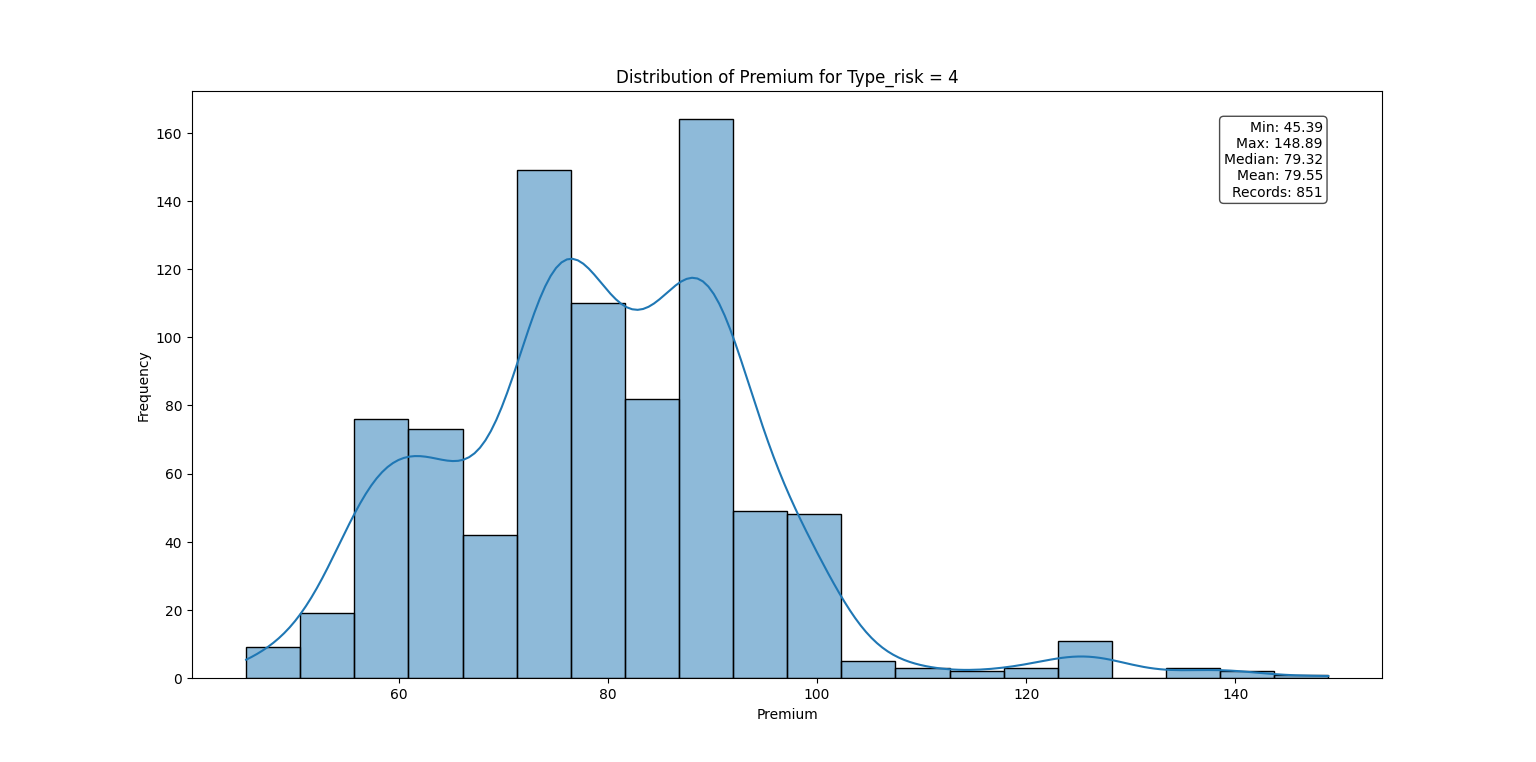
\includegraphics[width=\linewidth]{images/premium_risk4.png}
        \caption{Agricultural Vehicles}
        \label{fig:subfig4}
         \end{subfigure}
  \caption{Comparison of Different Vehicle Types}
  \label{fig:subfigures4}
\end{figure}



\begin{observation}
    Στο πρώτο διάγραμμα παρουσιάζεται η κατανομή των ασφαλίστρων για όλες τις καταχωρίσεις. Τα επόμενα διαγράμματα δείχνουν την κατανομή των ασφαλίστρων για κάθε κατηγορία οχημάτων ξεχωριστά.

    Εύκολα διαπιστώνεται από το πρώτο ολικό διάγραμμα ότι οι ασφαλιστικές τιμές πάνω από 500 είναι ελάχιστες και δεν επηρεάζουν σημαντικά το τελικό αποτέλεσμα. Ωστόσο, όταν κατηγοριοποιήσαμε τα δεδομένα, παρατηρήσαμε ότι η διασπορά των τιμών στα αγροτικά οχήματα ήταν μεγαλύτερη, με αποτέλεσμα η διαφοροποίηση του μοντέλου ανά κατηγορία οχήματος να είναι απαραίτητη.
\end{observation}


\end{document}

